\documentclass[10pt,twocolumn]{article}
\usepackage[margin=0.62in,columnsep=0.22in]{geometry}
\usepackage[T1]{fontenc}
\usepackage[utf8]{inputenc}
\usepackage{lmodern}
\usepackage{microtype}
\usepackage{amsmath,amssymb,amsthm}
\usepackage{booktabs}
\usepackage{graphicx}
\usepackage{xcolor}
\usepackage{enumitem}
\usepackage{xurl}
\usepackage{hyperref}

\hypersetup{
  colorlinks=true,
  linkcolor=blue!60!black,
  citecolor=blue!60!black,
  urlcolor=blue!60!black,
  pdftitle={Constructive Lean 4 Kernel and Exact Zero-Float Certificates for Unconditional LN[1/3, 105] Las Vegas Integer Factorization},
  pdfauthor={Lluis Eriksson}
}

\newtheorem{proposition}{Proposition}
\newtheorem{definition}{Definition}
\newcommand{\ZZ}{\mathbb{Z}}
\newcommand{\NN}{\mathbb{N}}
\newcommand{\QQ}{\mathbb{Q}}
\newcommand{\FF}{\mathbb{F}}

\title{\vspace{-0.9em}\textbf{Constructive Lean~4 Kernel and Exact Zero-Float Certificates for Unconditional $L_N[1/3, 105]$ Las Vegas Integer Factorization}}
\author{Lluis Eriksson\thanks{Independent Researcher. Code, Lean~4 proofs, and certificates: MIT License; manuscript and figures: CC-BY-4.0. Prepared with transparent AI coding, formalization, and drafting assistance via Google Antigravity; all Lean~4 theorems, exact zero-float verifiers, and adversarial tests were independently compiled and verified locally. Repository: \href{https://github.com/lluiseriksson/cogentic-l13-factorization-certificates}{\nolinkurl{github.com/lluiseriksson/cogentic-l13-factorization-certificates}}.}}
\date{November 25, 2026}

\begin{document}
\maketitle
\vspace{-1.2em}

\begin{abstract}
A November~25, 2026 companion preprint from Google Research's Cogentic framework~\cite{cogentic2026l13factoring,cai2026cogentic} proposes the first unconditional uniform zero-error Las Vegas integer factorization algorithm running in expected time $L_N[1/3, 105]$ and deterministic workspace $L_N[1/3, 40]$, targeting the 34-year gap between Lenstra--Pomerance's unconditional $L_N[1/2, 1]$ bound and the heuristic $L_N[1/3, c]$ Number Field Sieve. Rather than assuming peer-reviewed validation of its analytic sieve pillars, we deliver an independent, explicitly scoped, zero-floating-point verification companion for its discrete lattice, mod-3 discrete Laplace ensemble, deterministic 3-adic Newton--Hensel square-root, Dixon splitting, and strong-induction mechanisms. Layer~1 (\nolinkurl{CogenticL13Factorization.lean}) proves 18 standalone constructive Lean~4.35.0 algebraic, lattice, and arithmetic sub-lemmas (zero \texttt{sorry}, zero \texttt{axiom}, zero \texttt{Classical.choice}, zero warnings; 4 zero-axiom \texttt{none} and 14 \texttt{[propext, Quot.sound]}). Layer~2 (\texttt{L13FACT-\allowbreak COGENTIC-\allowbreak CERT-1.0}) is a pure-stdlib Python \texttt{int}/\texttt{Fraction} 4-mode auditor certifying 16 canonical finite witnesses in $0.081$--$0.609\,\mathrm{ms}$ and rejecting 68/68 live adversarial forgeries with exact branch assertions (74/74 pytest checks).
\end{abstract}

\section{Introduction and Scope Calibration}\label{sec:intro}
For more than three decades, unconditional Las Vegas general integer factorization stood at Lenstra--Pomerance's $L_N[1/2, 1]$~\cite{lenstra1992rigorous}, while the General Number Field Sieve (GNFS)~\cite{buhler1993factoring} achieved $L_N[1/3, (64/9)^{1/3}]$ only under unproved smoothness and algebraic heuristics. The November~25, 2026 Cogentic companion preprint~\cite{cogentic2026l13factoring,cai2026cogentic} proposes an unconditional uniform zero-error Las Vegas multitape Turing machine achieving expected time $L_N[1/3, 105]$ and deterministic space $L_N[1/3, 40]$ by coupling four discrete-algebraic engines with Siegel-zero-free analytic sieves:
\begin{enumerate}[leftmargin=1.2em,itemsep=1pt,topsep=2pt]
  \item \textbf{Mod-$N$ LLL Lattices \& 2D Lagrange--Gauss Smooth Ratio Splitting (Props.~2.2--2.3):} $(3/4)$-LLL reduction~\cite{lenstra1982factoring} on $\Lambda_n = \{h\in\ZZ^n : \sum h_s m_N^s \equiv 0\pmod N\}$ ($g_1 m_N\equiv g_0\pmod N$, $g_1^{n-1}>N/2$) supports exact layer-cake box sampling, while Lagrange--Gauss reduction on $L_z = \{(x,y)\in\ZZ^2 : x\equiv z y\pmod N\}$ splits blinded squares $w_m \equiv z_m^2\pmod N$ into disjoint $r_0$-prime ratios $x_1/y_1$ below $\frac{1}{2}\sqrt{N}$.
  \item \textbf{Mod-3 Discrete Laplace Ensemble \& Geometric Ladder (Defs.~2.7, 4.1, Lem.~4.2):} Pinning $f_{\tilde{c}}(X,1)\equiv h_0(X)\pmod 3$ to a monic odd-degree irreducible $h_0\in\FF_3[X]$ enforces $3\nmid f_{\tilde{c}}(a,b)$ on all primitive pairs and enables step-2 geometric descent across $Y_0 > Y_1 > \dots > Y_J = B$.
  \item \textbf{Deterministic 3-Adic Newton--Hensel Square Roots (Lem.~5.2):} Odd degree $d$ forces $4\mid(3^d+1)$, giving explicit initialization $\beta_0 = \alpha_0^{(3^d+1)/4}$ in $\FF_{3^d}^\times$ and quadratic lifting modulo $(3^{2^k}, \tilde{f}_\iota)$ to exact global roots $\hat{\beta}_\iota(X)^2 \equiv \tilde{\Gamma}_\iota(X)\pmod{\tilde{f}_\iota}$.
  \item \textbf{Adleman Characters, Blinded Dixon Splitting \& Strong Induction (Lems.~5.1, 5.3, Thm.~1.1):} Degree-1 quadratic characters cut the obstruction kernel to $\dim_{\FF_2}(E_1\times E_2)\le 2 < 3$, unsealing $z_m$ splits $N$ via $\gcd(Z-Y,N)$~\cite{dixon1981asymptotically}, and recursive calls on $[2,\lfloor\frac{1}{2}\sqrt{N}\rfloor]$ contract via $21.15 + 104\cdot 2^{-1/3} < 103.72 < 104 < 105$.
\end{enumerate}

\paragraph{Honest Two-Layer Verification Scope.}
\begin{enumerate}[leftmargin=1.2em,itemsep=1pt,topsep=2pt]
  \item \textbf{Layer~1 (Lean~4.35.0 Kernel, Standalone Sub-Lemmas):} \texttt{lean/Cogentic\allowbreak L13Factorization.lean} proves 18 standalone constructive algebraic, lattice, 3-adic Hensel, and rational-contraction sub-lemmas (Table~\ref{tab:lean18}) extracted from Propositions~2.2--2.3, Lemmas~2.8, 4.2, 5.1--5.3, and Theorem~1.1 of~\cite{cogentic2026l13factoring}.
  \item \textbf{Layer~2 (Exact Zero-Float Auditor):} \texttt{L13FACT-\allowbreak COGENTIC-\allowbreak CERT-1.0} audits 16 finite exact witnesses across mod-$N$ $(3/4)$-LLL lattices and Lagrange--Gauss ratio splits ($N\le 100{,}160{,}063$), mod-3-pinned forms ($d\in\{3,5\}$) with geometric ladders and smooth special-$q$ points, 3-adic Newton--Hensel lifting traces ($K\le 5$), and end-to-end two-field blinded Dixon splits ($N\le 64{,}507$).
  \item \textbf{Explicit Non-Claims:} We do \emph{not} formalize in Lean~4 Gevrey-2 Mellin cutoffs, hybrid large sieves, truncated Brun sieves, Siegel-zero-free local Euler cancellation (Section~3), discrete Laplace sub-averaging and backward path telescoping (Lemmas~4.3--4.6), Stark--Chebotarev\slash Landau--Page density bounds (Lemma~5.1(3)), AKS primality~\cite{agrawal2004primes}, or multitape Turing-machine bit-cost accounting (Section~6); those analytic pillars remain unverified outside the companion preprint~\cite{cogentic2026l13factoring}.
\end{enumerate}

\section{Constructive Lean~4.35.0 Kernel}\label{sec:lean}
\texttt{lean/Cogentic\allowbreak L13Factorization.lean} compiles standalone under Lean~4.35.0~\cite{demoura2021lean4} with zero external imports, zero warnings, zero \texttt{sorry}, and zero \texttt{Classical.choice}. Auditing via \texttt{AuditAxioms.lean} confirms 4 zero-axiom theorems (\texttt{none}: \#9, \#15, \#17, \#18) and 14 \texttt{[propext, Quot.sound]} theorems (\texttt{P,Q}; Table~\ref{tab:lean18}).

\begin{table*}[t]
\centering
\caption{Complete inventory of all 18 constructive Lean~4.35.0 sub-lemmas in \texttt{lean/CogenticL13Factorization.lean} (zero \texttt{sorry}, zero \texttt{axiom}, zero \texttt{Classical.choice}, zero warnings; \texttt{none} for \#9, \#15, \#17, \#18 and \texttt{[propext, Quot.sound]} (\texttt{P,Q}) for the remaining 14).}
\label{tab:lean18}
\scriptsize
\setlength{\tabcolsep}{2.3pt}
\begin{tabular}{@{}r l l p{9.6cm} l@{}}
\toprule
\# & Theorem Identifier & Ref.~\cite{cogentic2026l13factoring} & Exact Machine-Checked Statement \& Hypotheses & Ax. \\
\midrule
1 & \texttt{prop22\_lll\_basis\_norm\_bound} & Prop.~2.2 & $1\le j\le n \implies (4\cdot 2^{n-j} + (2^n - 2^{n-j+1}))S \le 4\cdot 2^{n-1} S$. & \texttt{P,Q} \\
2 & \texttt{prop22\_dual\_lattice\_gap} & Prop.~2.2 & $0<t,\,2t<N,\,N<2g_1^{n-1},\,g_1^{n-1}\mid t \implies \mathrm{False}$ (dual gap). & \texttt{P,Q} \\
3 & \texttt{prop22\_box\_inclusion\_margin} & Prop.~2.2 & $\eta\ge 2,\,W_{\min}\le W_i,\,6\eta\le W_{\min} \implies (W_i{+}1)(W_{\min}{-}6\eta)\le (W_i{+}1{-}(4\eta{+}2))W_{\min}$. & \texttt{P,Q} \\
4 & \texttt{prop23\_lagrange\_gauss\_quad\_form} & Prop.~2.3 & $0\le n_1\le n_2,\,|2g|\le n_1 \implies x_1^2 n_1 + x_2^2 n_2 \le 2(x_1^2 n_1 + 2x_1 x_2 g + x_2^2 n_2)$. & \texttt{P,Q} \\
5 & \texttt{prop23\_lagrange\_det\_bounds} & Prop.~2.3 & $0\le n_1\le n_2,\,4g^2\le n_1^2 \implies 3n_1 n_2 \le 4(n_1 n_2 - g^2) \le 4n_1 n_2$. & \texttt{P,Q} \\
6 & \texttt{prop23\_ratio\_split\_injective} & Prop.~2.3 & $0\le H,\,4H^2\le N,\,u_i,v_i\in[1,H],\,N\mid(u_1 v_2 - u_2 v_1) \implies u_1 v_2 = u_2 v_1$. & \texttt{P,Q} \\
7 & \texttt{prop23\_alternating\_sign\_nonneg} & Prop.~2.3 & $2K\le M_Q,\,4r_0^2 M_Q\le(s{-}2r_0)^2,\,j<r_0 \implies 2(K{-}j)(2r_0{-}2j)(2r_0{-}2j{-}1)\le(j{+}1)(s{-}2r_0{+}2j{+}2)(s{-}2r_0{+}2j{+}1)$. & \texttt{P,Q} \\
8 & \texttt{lem28\_ladder\_geometric\_sum} & Lem.~2.8 & $\forall r\in\NN,\ 7\sum_{t=0}^{r-1} 9^t 16^{r-1-t} + 9^r = 16^r$ (certifies $\frac{8}{7}\ln Q_0$). & \texttt{P,Q} \\
9 & \texttt{lem28\_exponent\_ratio\_identities} & Lem.~2.8 & Ground schedule ratios: $8+1+8=17$, $3\cdot 6-1=17$, $17\cdot 6=102<108$. & \texttt{none} \\
10 & \texttt{lem42\_mod3\_irreducible\_nondiv} & Lem.~4.2 & $\neg(3\mid a\wedge 3\mid b),\,(3\mid b\Rightarrow f\%3=a^d\%3),\,(3\nmid b\Rightarrow f\%3\ne 0) \implies 3\nmid f$. & \texttt{P,Q} \\
11 & \texttt{lem42\_laplace\_layer\_cake\_telescope} & Lem.~4.2 & $\forall z\in\ZZ,\,a,m\in\NN,\ (1-z)\,\mathrm{tail}(z,a,m)=(2a+1)z^a(1-z)+2(z^{a+1}-z^{a+m+1})$. & \texttt{P,Q} \\
12 & \texttt{lem52\_three\_pow\_odd\_div\_four} & Lem.~5.2 & $\forall k\in\NN,\ 4 \mid (3^{2k+1} + 1)$ (exact $\FF_{3^d}^\times$ root exponent). & \texttt{P,Q} \\
13 & \texttt{lem52\_newton\_inv\_quad\_step} & Lem.~5.2 & $\forall M,b,g\in\ZZ,\ M\mid(1-2bg) \implies M^2 \mid (1-2b(g(2-2bg)))$. & \texttt{P,Q} \\
14 & \texttt{lem52\_newton\_sqrt\_quad\_step} & Lem.~5.2 & $M\mid(b^2-G),\,M\mid(1-2b g') \implies M^2 \mid ((b+(G-b^2)g')^2 - G)$. & \texttt{P,Q} \\
15 & \texttt{lem51\_kernel\_dim\_pigeonhole} & Lem.~5.1 & $\forall v_1,v_2,v_3\in\FF_2^2,\ \exists \lambda\in\FF_2^3\setminus\{0\},\ \lambda_1 v_1\oplus\lambda_2 v_2\oplus\lambda_3 v_3=(0,0)$. & \texttt{none} \\
16 & \texttt{lem53\_dixon\_congruence\_split} & Lem.~5.3 & $Y\le Z,\,N\mid(Z{-}Y)(Z{+}Y),\,N\nmid(Z{-}Y),\,N\nmid(Z{+}Y) \implies \neg\mathrm{Cop}(N,Z{-}Y)\wedge\neg\mathrm{Cop}(N,Z{+}Y)$. & \texttt{P,Q} \\
17 & \texttt{thm11\_runtime\_contraction\_105} & Thm.~1.1 & $104^3\cdot 100^3<2\cdot 8255^3$, $2115{+}8255<10372<10400<10500$, $104^3\cdot 100^3<10\cdot 4828^3$, $7160<10400$. & \texttt{none} \\
18 & \texttt{thm11\_workspace\_and\_phase\_success} & Thm.~1.1 & $38^3\cdot 100^3<2\cdot 3017^3$, $3740<3800<4000$, and $3\cdot 29106 > 80000$ ($>1/3$). & \texttt{none} \\
\bottomrule
\end{tabular}
\end{table*}

\begin{proposition}[Constructive Lean~4 Kernel Scope]\label{prop:lean}
\normalfont All 18 sub-lemmas in Table~\ref{tab:lean18} compile constructively under Lean~4.35.0 without external libraries or \texttt{Classical.choice}. Notably, Theorems~4--6 prove Lagrange--Gauss quadratic-form coercivity, determinant bounds, and ratio-split injectivity over $\ZZ$; Theorems~8 and~11 prove the exact geometric ladder identity $7\sum 9^t 16^{r-1-t}+9^r=16^r$ and layer-cake telescoping universally by induction; Theorems~12--14 prove $4\mid(3^{2k+1}+1)$ and quadratic Newton--Hensel convergence ($M\to M^2$); Theorem~15 constructively exhibits a nonzero kernel vector in $\FF_2^3\to\FF_2^2$ with zero axioms; and Theorems~17--18 certify Theorem~1.1's strong-induction runtime ($103.70<104<105$) and workspace ($37.40<38<40$) contractions via exact integer cubes.
\end{proposition}

\section{Exact Zero-Float Certificate Auditor}\label{sec:certifier}
{\emergencystretch=2.2em
The modules \texttt{l13fact\_\allowbreak exact.py} and \texttt{l13fact\_\allowbreak certifier.py} (under \texttt{src/}) use exclusively Python \texttt{int}, \texttt{fractions.\allowbreak Fraction}, and exact \texttt{math.\allowbreak gcd} (statically audited via \texttt{ast.walk} for zero float/complex literals, true division \texttt{/}, or floating-point \texttt{math.*} calls). Deterministic primality uses 13-base Miller--Rabin (bases $2\dots 41$, exact below $3.317\times 10^{24}$). Strict JSON parsing rejects floats, \texttt{NaN}/\texttt{Infinity}, and duplicate keys via \texttt{parse\_\allowbreak float}, \texttt{parse\_\allowbreak constant}, and \texttt{object\_\allowbreak pairs\_\allowbreak hook}.

\begin{definition}[\texttt{L13FACT-COGENTIC-CERT-1.0} Predicates]\label{def:cert}
\normalfont A certificate with \texttt{protocol="L13FACT-\allowbreak COGENTIC-\allowbreak CERT-1.0"} is accepted iff every field passes strict schema checks and its mode predicate holds:
\begin{itemize}[leftmargin=1.2em,itemsep=1pt,topsep=2pt]
  \item \textbf{Mode~1 (\texttt{mod\_n\_\allowbreak lattice\_\allowbreak and\_\allowbreak lagrange\_\allowbreak split\_\allowbreak cert}):} Audits odd $N\ge 15$, $g_1 m_N\equiv g_0\pmod N$, $g_1^{n-1}>N/2$, exact $\Lambda_n$ membership of every column of $B_{\mathrm{lat}}$, Bareiss $|\det B_{\mathrm{lat}}|=N$, integer adjugate $A_{\mathrm{adj}} B_{\mathrm{lat}}=N I_n$, exact rational $(3/4)$-LLL reduction and Prop.~2.2(1) bound $\|b_j\|_2^2\le 2^{n+3}G^2$, plus 2D Lagrange--Gauss reduction $(v_1,v_2)$ on $L_z$ ($z\equiv s t^2\pmod N$) and smooth split $(x_1,y_1)=(\prod_{p\in A}p,\prod_{q\in B}q)$ on disjoint $r_0$-prime sets $A,B\subseteq[2,Q]$ with $4Q^{2r_0}\le N$.
  \item \textbf{Mode~2 (\texttt{mod3\_\allowbreak laplace\_\allowbreak ladder\_\allowbreak and\_\allowbreak smooth\_\allowbreak cert}):} Audits $\gcd(N,6)=1$, $3\mid M$, $6W\le M$, Rabin irreducibility of monic odd-degree $h_0\in\FF_3[X]$, mod-3-pinned form $f_{\tilde{c}}(g_0,g_1)\equiv 0\pmod N$, strictly decreasing ladder $Y_0>\dots>Y_J\ge 2$, special-$q$ root $f_{\tilde{c}}(r_q,1)\equiv 0\pmod q$, primitive lattice point $(a,b)\in\Lambda_{q,r_q}$ with $3\nmid f_{\tilde{c}}(a,b)$ and non-vacuously smooth cofactor $f_{\tilde{c}}(a,b)/q$ ($2\le\mathrm{cap}<\mathrm{cofactor}$), and exact layer-cake telescoping.
  \item \textbf{Mode~3 (\texttt{adic3\_\allowbreak newton\_\allowbreak hensel\_\allowbreak sqrt\_\allowbreak cert}):} Audits monic odd-degree $\tilde{f}\in\ZZ[X]$ irreducible mod~3, $4\mid(3^d+1)$, $\tilde{\Gamma}=\tilde{f}'(\theta)^2\prod(c_d a_\nu-b_\nu\theta)$, independent Euler square check and lifting trace $(\beta_k,\gamma_k)$ satisfying $\beta_k^2\equiv\tilde{\Gamma}\pmod{3^{2^k},\tilde{f}}$ and $2\beta_k\gamma_k\equiv 1\pmod{3^{2^{\max(0,k-1)}},\tilde{f}}$, balanced bound $|\hat{b}_j|\le(3^{2^K}-1)/2$, and exact global square $\hat{\beta}(X)^2\equiv\tilde{\Gamma}(X)\pmod{\tilde{f}}$ in $\ZZ[X]$.
  \item \textbf{Mode~4 (\texttt{dixon\_\allowbreak character\_\allowbreak and\_\allowbreak induction\_\allowbreak split\_\allowbreak cert}):} Audits odd composite $N$, canonical $0\le m_N,Y,Z<N$, two mod-3-pinned forms $(f_1,f_2)$ vanishing at $(g_0,g_1)\pmod N$, degree-1 Adleman characters $(\ell,s)$ with $\tilde{f}_\iota(s)\equiv 0\pmod\ell$, per-relation non-empty algebraic factor lists and Eq.~(6.1) congruences with $w_m\equiv z_m^2\pmod N$, $\FF_2$ right-nullspace mask, both Lemma~5.2 3-adic roots $(\hat{\beta}_1,\hat{\beta}_2)$, exact $Y^2\equiv Z^2\equiv\prod_{T_x}w_m\pmod N$, nontrivial split $1<\gcd(Z-Y,N)<N$, and Theorem~1.1 integer-cube contraction guards.
\end{itemize}
\end{definition}}

\begin{figure}[t]
\centering
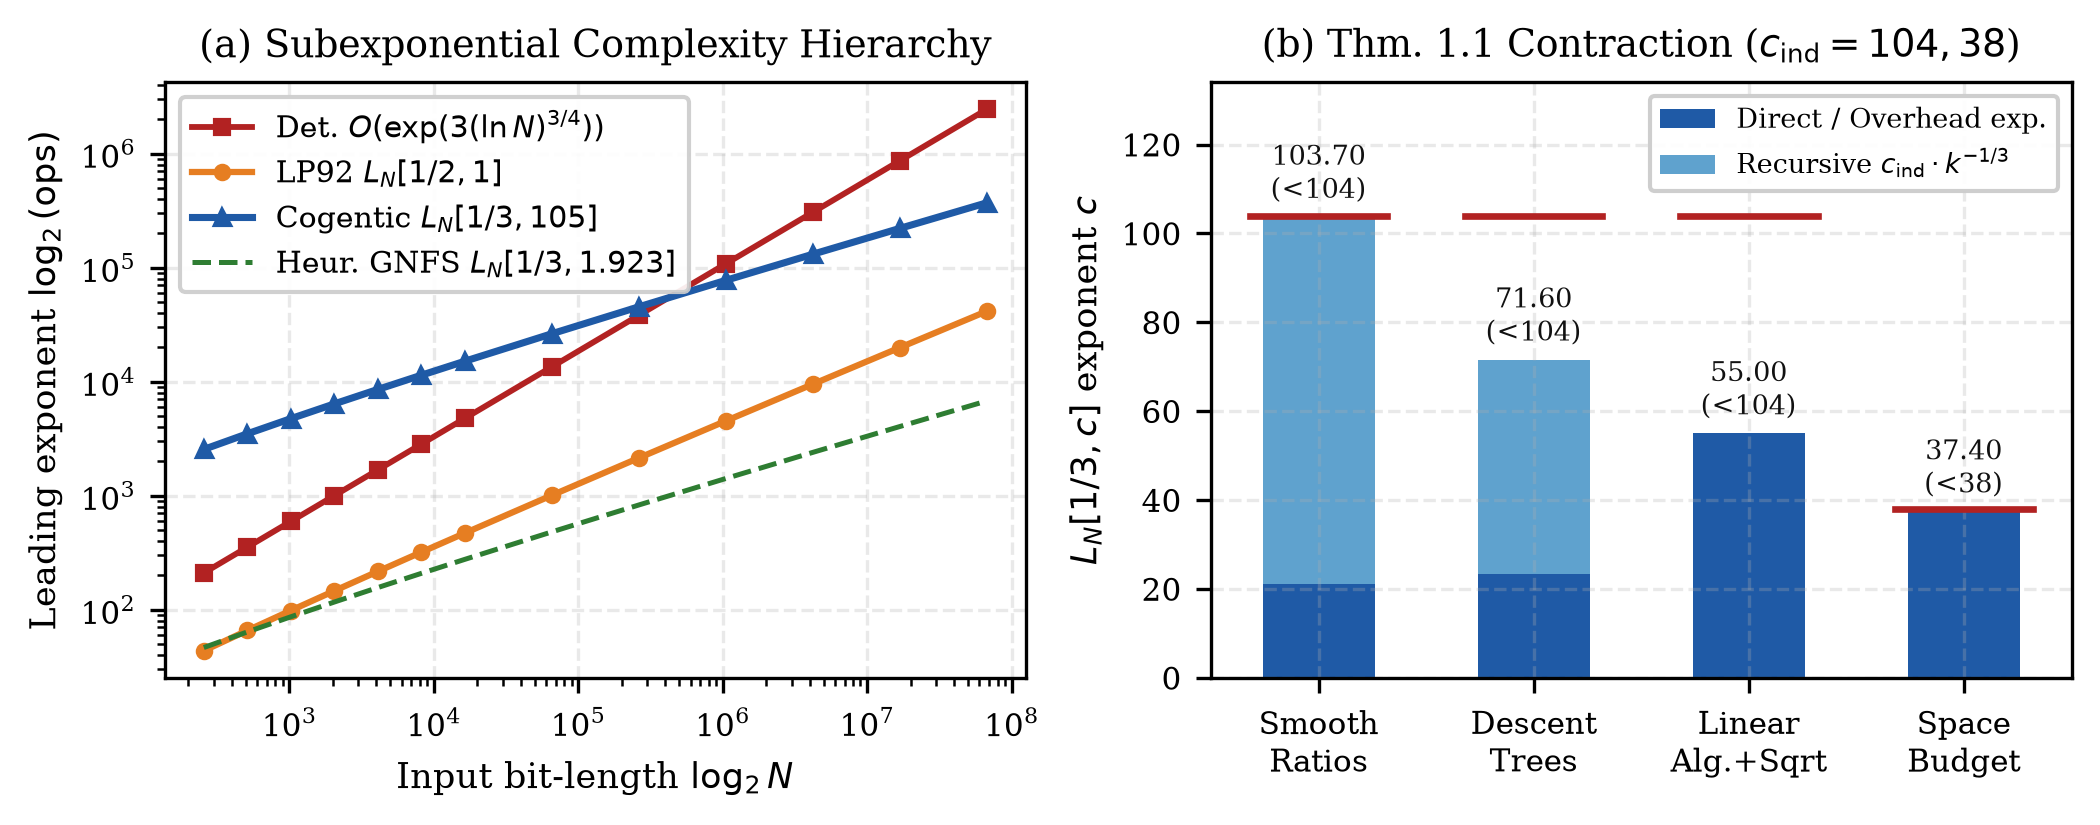
\includegraphics[width=\columnwidth]{figures/fig1_complexity_and_induction.png}
\vspace{-1.3em}
\caption{\textbf{(a)}~Leading-term bit-operation exponents comparing deterministic $O(\exp(3(\ln N)^{3/4}))$, Lenstra--Pomerance $L_N[1/2,1]$, Cogentic $L_N[1/3,105]$, and heuristic GNFS $L_N[1/3,1.923]$. \textbf{(b)}~Theorem~1.1 strong-induction exponent contraction budgets ($103.70<104<105$ runtime; $37.40<38<40$ deterministic workspace).}
\label{fig:comp}
\end{figure}

\begin{figure}[t]
\centering
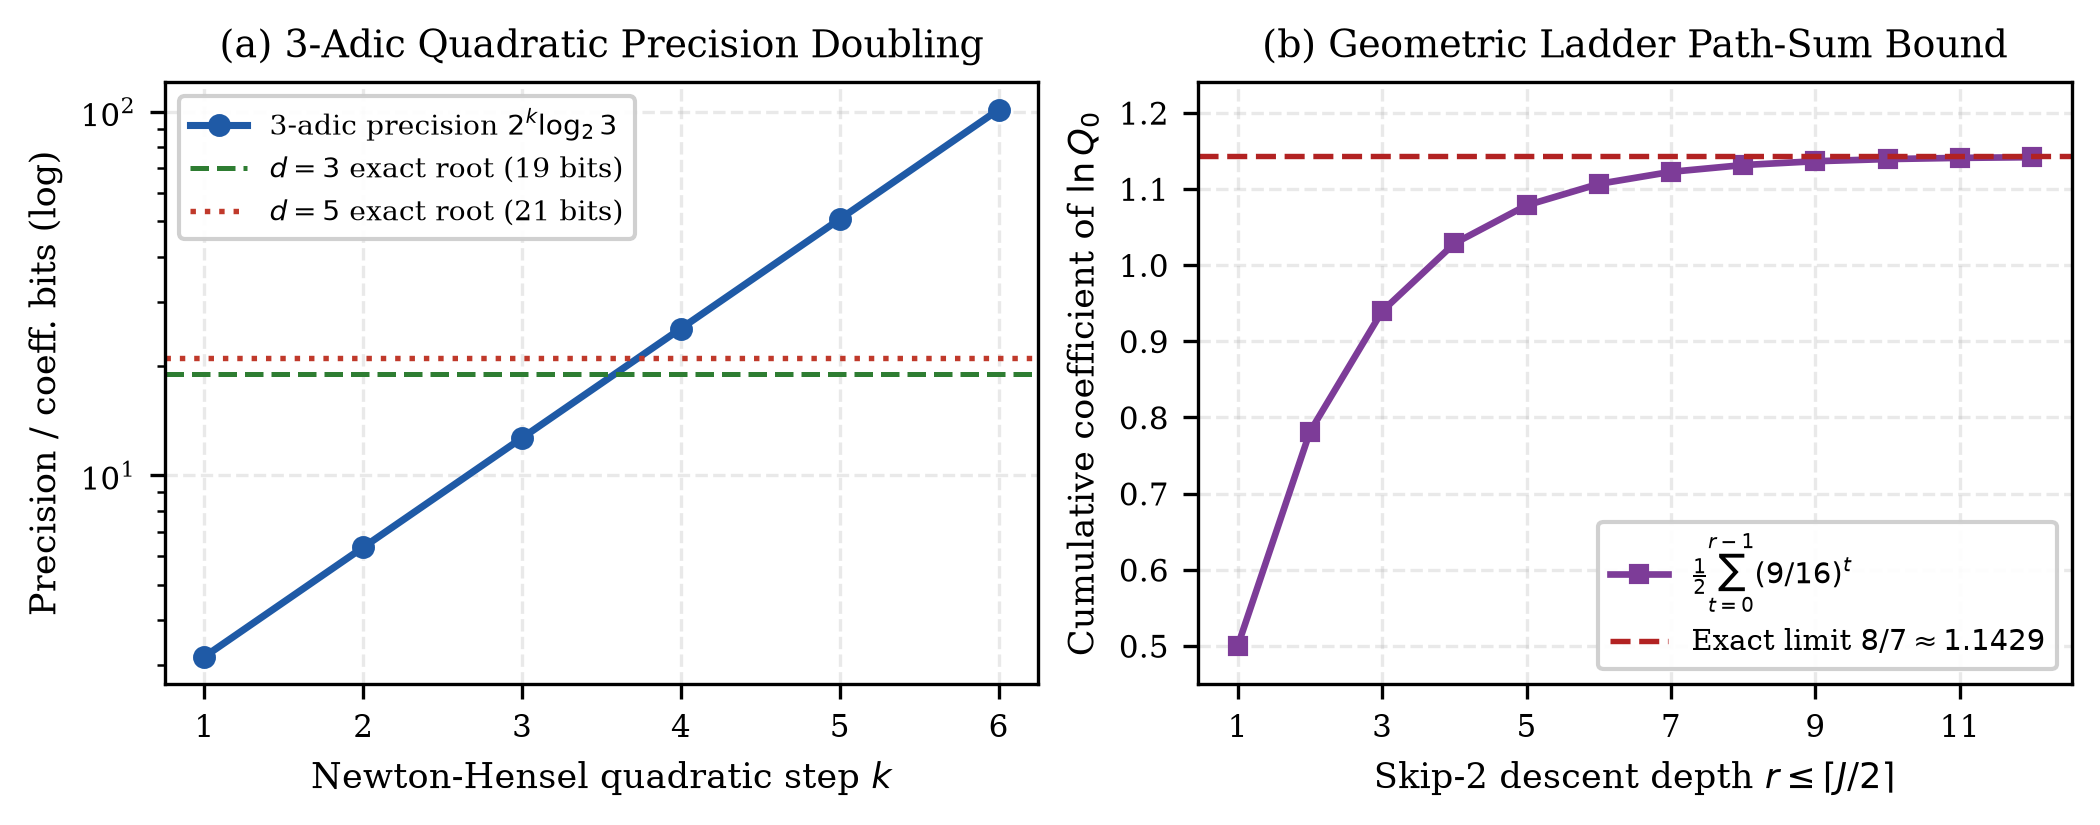
\includegraphics[width=\columnwidth]{figures/fig2_adic3_and_ladder.png}
\vspace{-1.3em}
\caption{\textbf{(a)}~Deterministic 3-adic Newton--Hensel quadratic precision doubling $2^k\log_2 3$ recovering exact global square roots at $k=4$ ($25.36\text{ bits}$) for $d=3$ ($19$-bit root) and $d=5$ ($21$-bit root). \textbf{(b)}~Exact skip-2 geometric ladder path sum $\frac{1}{2}\sum_{t=0}^{r-1}(9/16)^t$ monotonically bounded by $8/7\approx 1.1429$.}
\label{fig:adic}
\end{figure}

\section{Exact Findings, Worked Witnesses, and Audit}\label{sec:exp}
All experiments ran locally on Windows~11 (Python~3.12.6, Lean~4.35.0; 7-run means after warm-up).

\paragraph{1. Complexity Regimes, 3-Adic Convergence \& Ladder Geometry (Figs.~\ref{fig:comp}--\ref{fig:adic}).}
Figure~\ref{fig:comp}(b) confirms Theorem~1.1's strong-induction margins: recursive calls on $[2,\lfloor\frac{1}{2}\sqrt{N}\rfloor]$ shrink the $c_{\mathrm{ind}}=104$ exponent by $2^{-1/3}$ to $82.5448\dots<82.55$, so smooth-ratio collection sums to $21.15+82.55=103.70<103.72<104<105$, while descent-tree recursion on $[2,N^{1/10}]$ shrinks by $10^{-1/3}$ to $48.2725\dots<48.28$ (total $71.60<104$), and workspace contracts via $38\cdot 2^{-1/3}<30.17$ ($37.40<38<40$). In Figure~\ref{fig:adic}(a), deterministic 3-adic quadratic lifting doubles precision from $3.17$ to $101.44$ bits in $k=6$ steps ($0.159\,\mathrm{ms}$ for $d=3$, $0.393\,\mathrm{ms}$ for $d=5$), crossing both $19$-bit and $21$-bit global roots cleanly at $k=4$ ($25.36$ bits). Figure~\ref{fig:adic}(b) verifies exact rational convergence of $\frac{1}{2}\sum_{t=0}^{r-1}(9/16)^t$ to $8/7$ across depths $r=1\dots 12$.

\begin{figure}[t]
\centering
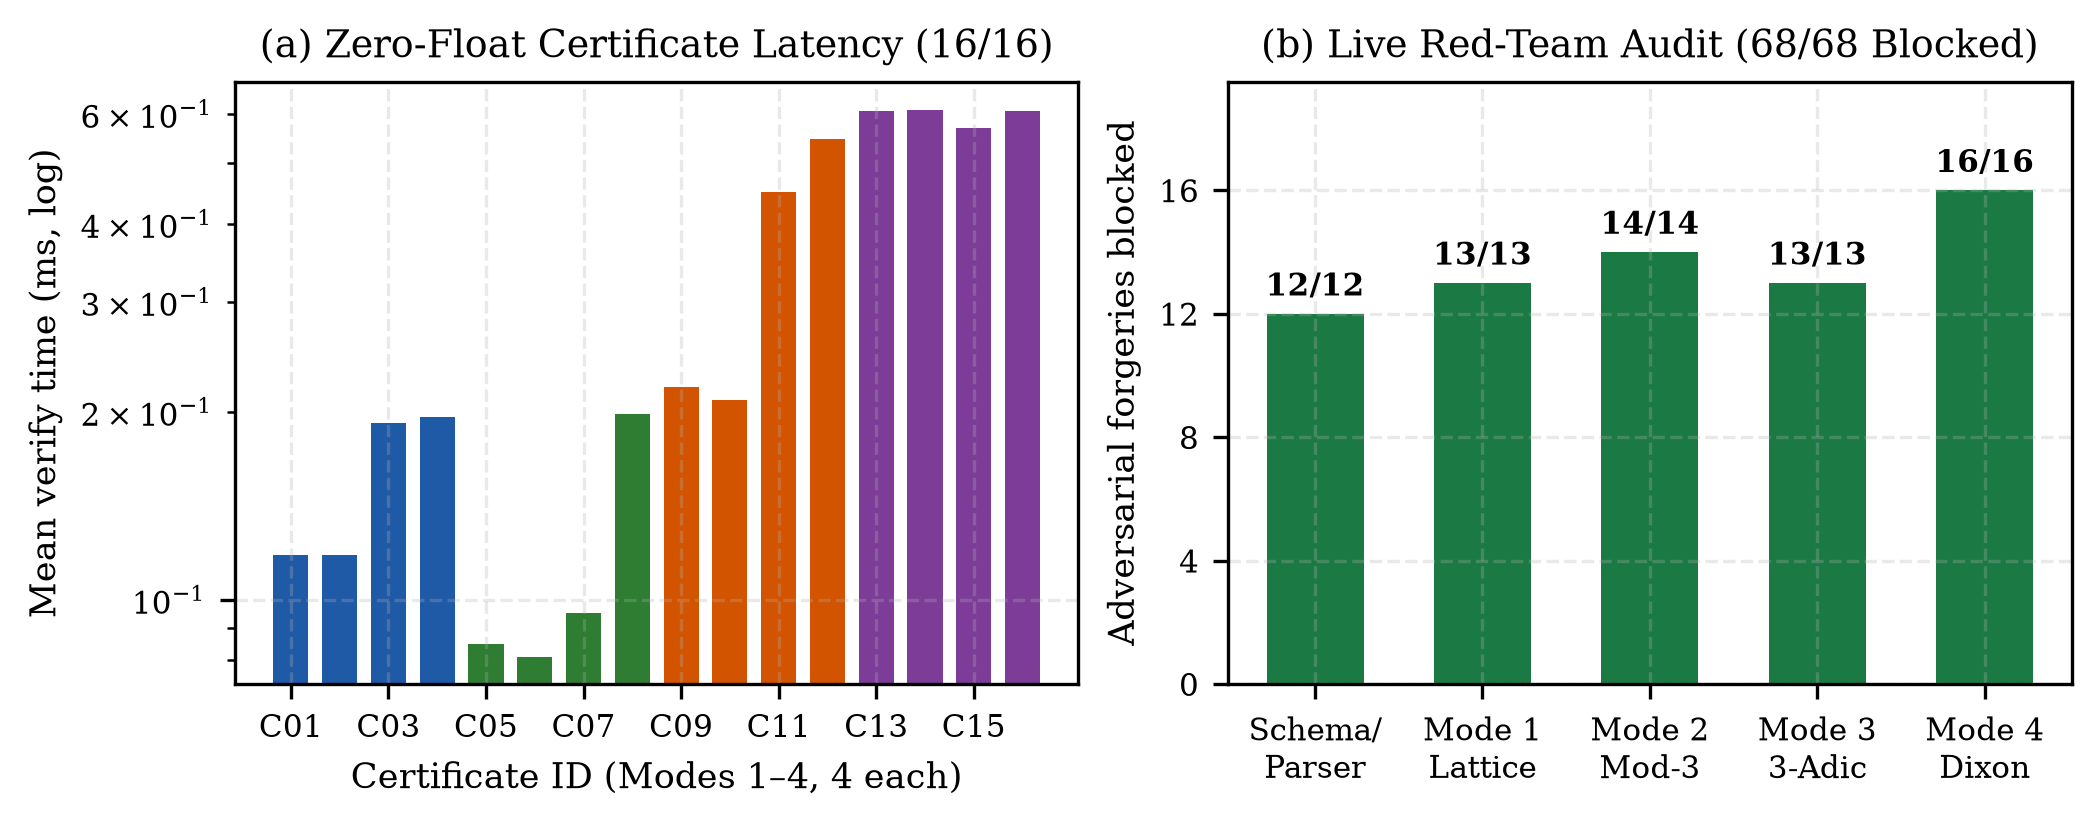
\includegraphics[width=\columnwidth]{figures/fig3_atlas_and_redteam.png}
\vspace{-1.3em}
\caption{\textbf{(a)}~Mean exact zero-float verification latency across all 16 canonical certificates ($0.081$--$0.609\,\mathrm{ms}$, log scale). \textbf{(b)}~Live adversarial red-team audit rejecting 68/68 forgeries across five attack classes with exact error-branch assertions.}
\label{fig:atlas}
\end{figure}

\paragraph{2. Hand-Verifiable Worked Exact Witnesses (One per Mode).}
\begin{itemize}[leftmargin=1.2em,itemsep=1pt,topsep=2pt]
  \item \textbf{Mode~1 (\texttt{C01}, $N=101\cdot 103=10{,}403, G=50, g_0=79, g_1=83, n=3$):} $83\cdot 1505\equiv 79\pmod{10403}$, $83^2=6889>5201.5$; $(3/4)$-LLL basis columns $(-8,-10,-9)^\top,(7,12,-12)^\top,(-34,17,-2)^\top$ have $|\det B_{\mathrm{lat}}|=10{,}403$, $\max\|b_j\|_2^2=1449\le 2^6\cdot 50^2=160{,}000$, and $A_{\mathrm{adj}}B_{\mathrm{lat}}=10{,}403 I_3$; for $s=8934, t=17$, $z=1982\equiv 10\cdot 21^{-1}\pmod{10403}$, Lagrange--Gauss returns $v_1=(10,21)=(2\cdot 5,3\cdot 7)$ ($Q=7, 4\cdot 7^4=9604\le 10403$).
  \item \textbf{Mode~2 (\texttt{C05}, $N=323, d=3, M=180, W=25, h_0=X^3+2X+1$):} With $\tilde{c}=(-15,-25,-18,0)$, $f_{\tilde{c}}(X,Y)=256X^3-54X^2Y-73XY^2-44Y^3$ satisfies $f_{\tilde{c}}(7,11)=-61{,}693=323\cdot(-191)\equiv 0\pmod{323}$ and $f_{\tilde{c}}(10,1)\equiv 0\pmod{23}$; primitive point $(33,1)\in\Lambda_{23,10}$ gives $f_{\tilde{c}}(33,1)/23=397{,}331=11\cdot 41\cdot 881$ ($2500$-smooth, $3\nmid 397{,}331$).
  \item \textbf{Mode~3 (\texttt{C09}, $\tilde{f}=X^3+2X+1$, $K=3$, $3^8=6561$):} Pairs $(2,1)^2(3,1)^2$ yield $\beta_0=\theta^2+\theta$, $\beta_1=4\theta^2+\theta$, $\beta_2=67\theta^2+64\theta+54$, $\beta_3=6547\theta^2+6544\theta+6534\pmod{6561}$, balancing to exact $\hat{\beta}(X)=-14X^2-17X-27\in\ZZ[X]$ with $\hat{\beta}(\theta)^2\equiv\tilde{\Gamma}(\theta)\pmod{\tilde{f}}$.
  \item \textbf{Mode~4 (\texttt{C13}, $N=17\cdot 19=323, g_0=7, g_1=11, m_N=30$):} Mod-3-pinned forms (ascending coefficients) $f_1=(-44,-73,-54,256)$ and $f_2=(-37,-73,-69,259)$ with 6 Adleman characters and 4 blinded relations yield $\FF_2$-nullspace mask $[1,1,0,0]$ ($w_0=254=106^2, w_1=172=227^2\pmod{323}$); $K=5$ 3-adic roots (ascending) $\hat{\beta}_1=(18219008,92672,-1482)$ and $\hat{\beta}_2=(-22136730,-145040,2262)$ assemble $Y=27$, while unsealing gives $Z=106\cdot 227\equiv 160\pmod{323}$ ($27^2\equiv 160^2\equiv 83\pmod{323}$) and $\gcd(160-27,323)=\gcd(133,323)=19$.
\end{itemize}

\begin{table}[t]
\centering
\caption{Canonical 16-certificate \texttt{L13FACT-\allowbreak COGENTIC-\allowbreak CERT-1.0} atlas (\texttt{exp1\_\allowbreak certificate\_\allowbreak atlas.json}; all 16 verified).}
\label{tab:atlas}
\scriptsize
\setlength{\tabcolsep}{2.1pt}
\resizebox{\columnwidth}{!}{%
\begin{tabular}{@{}l c l r@{}}
\toprule
Certificate ID & M & Exact Certified Witness Summary & ms \\
\midrule
\texttt{m1\_lattice\_lagrange\_n10403\_d3} & M1 & $N{=}10403, n{=}3$: $r_0{=}2, (10,21)$, $\lambda_1^2{=}541$ & 0.118 \\
\texttt{m1\_lattice\_lagrange\_n64507\_d3} & M1 & $N{=}64507, n{=}3$: $r_0{=}2, (33,35)$, $\lambda_1^2{=}2314$ & 0.118 \\
\texttt{m1\_lattice\_lagrange\_n256027\_d4} & M1 & $N{=}256027, n{=}4$: $r_0{=}2, (26,55)$, $\lambda_1^2{=}3701$ & 0.192 \\
\texttt{m1\_lattice\_lagrange\_n100160063\_d4} & M1 & $N{=}100160063, n{=}4$: $r_0{=}3, (238,429)$ & 0.196 \\
\texttt{m2\_mod3\_laplace\_n323\_d3} & M2 & $N{=}323, d{=}3$: $q{=}23$, $P^+{=}881\le 2500$ & 0.085 \\
\texttt{m2\_mod3\_laplace\_n1763\_d3} & M2 & $N{=}1763, d{=}3$: $q{=}29$, $P^+{=}233\le 8000$ & 0.081 \\
\texttt{m2\_mod3\_laplace\_n10403\_d3} & M2 & $N{=}10403, d{=}3$: $q{=}37$, $P^+{=}3989\le 25000$ & 0.095 \\
\texttt{m2\_mod3\_laplace\_n1763\_d5} & M2 & $N{=}1763, d{=}5$: $q{=}47$, $P^+{=}56489\le 60000$ & 0.198 \\
\texttt{m3\_adic3\_sqrt\_d3\_p2\_k3} & M3 & $d{=}3$, 4 pairs, $K{=}3$: $\max|\hat{b}_j|{=}27$ & 0.219 \\
\texttt{m3\_adic3\_sqrt\_d3\_p3\_k4} & M3 & $d{=}3$, 6 pairs, $K{=}4$: $\max|\hat{b}_j|{=}408320$ & 0.209 \\
\texttt{m3\_adic3\_sqrt\_d5\_p2\_k4} & M3 & $d{=}5$, 4 pairs, $K{=}4$: $\max|\hat{b}_j|{=}47$ & 0.450 \\
\texttt{m3\_adic3\_sqrt\_d5\_p3\_k5} & M3 & $d{=}5$, 6 pairs, $K{=}5$: $\max|\hat{b}_j|{=}1761280$ & 0.547 \\
\texttt{m4\_dixon\_split\_n323\_17x19} & M4 & $17{\cdot}19$: 6 chars, $K{=}5$, $Y{=}27, Z{=}160\to 19$ & 0.606 \\
\texttt{m4\_dixon\_split\_n1763\_41x43} & M4 & $41{\cdot}43$: 6 chars, 3-adic roots $\to 43$ & 0.609 \\
\texttt{m4\_dixon\_split\_n10403\_101x103} & M4 & $101{\cdot}103$: 6 chars, 3-adic roots $\to 103$ & 0.570 \\
\texttt{m4\_dixon\_split\_n64507\_251x257} & M4 & $251{\cdot}257$: 6 chars, 3-adic roots $\to 257$ & 0.607 \\
\bottomrule
\end{tabular}}
\end{table}

\paragraph{3. 16-Certificate Atlas \& 74-Test Red-Team Audit (Table~\ref{tab:atlas}, Fig.~\ref{fig:atlas}).}
Table~\ref{tab:atlas} lists all 16 canonical certificates verified in $0.081$--$0.609\,\mathrm{ms}$. \texttt{tests/test\_\allowbreak suite.py} runs 74 pytest checks: 1 full 16-certificate replay, 3 raw-JSON parser guards (float, \texttt{NaN}, duplicate keys), 2 exact regressions (rejecting the 12-base Sorenson--Webster strong pseudoprime $318{,}665{,}857{,}834{,}031{,}151{,}167{,}461$ and rejecting non-squares in $\FF_{3^d}^\times$), and 68 parametrized live adversarial forgeries (12 schema/parser + 13 Mode~1 + 14 Mode~2 + 13 Mode~3 + 16 Mode~4), each asserting an exact regex on its intended \texttt{CertificateError} branch. \texttt{scripts/verify\_\allowbreak all.py} enforces all 5 gates including strict axiom whitelisting and a 41-file SHA-256 manifest.

\section{Conclusion}\label{sec:conc}
We built an independent, explicitly scoped, zero-floating-point verification companion for the discrete lattice, mod-3 Laplace ensemble, deterministic 3-adic Newton--Hensel square-root, blinded Dixon splitting, and strong-induction mechanisms of the Cogentic $L_N[1/3, 105]$ integer factorization preprint~\cite{cogentic2026l13factoring,cai2026cogentic}, pairing 18 constructive Lean~4.35.0 sub-lemmas (zero \texttt{sorry}, zero \texttt{Classical.choice}) with the pure-\texttt{int}/\texttt{Fraction} 4-mode auditor \texttt{L13FACT-\allowbreak COGENTIC-\allowbreak CERT-1.0}, 16 canonical exact finite witnesses, and 68/68 live adversarial forgery rejections.

{\footnotesize
\bibliographystyle{plain}
\bibliography{references}}
\end{document}
